\documentclass{beamer}
\usetheme{Madrid}
\usecolortheme{default}
\usepackage[T1]{fontenc}
\usepackage[utf8]{inputenc}
\usepackage{lmodern}
\usepackage{graphicx}
\usepackage{booktabs}
\usepackage{hyperref}

\title{UQ-QNN Rerun Experiments}
\subtitle{Memristor placement, multi-memristor tests, and backend speedups}
\author{Project Presentation}
\date{April 8, 2026}

\begin{document}

\begin{frame}
    \titlepage
\end{frame}

\begin{frame}{Repository Goal}
The repository studies uncertainty-aware photonic QNNs built on Clements meshes and memristive photonic circuits.

\vspace{0.5em}
Current goals:
\begin{itemize}
    \item train photonic models reproducibly,
    \item compare standard and memristive circuits,
    \item quantify uncertainty and calibration,
    \item make simulator reruns fast enough for architecture studies.
\end{itemize}
\end{frame}

\begin{frame}{Development Stages}
Recent progress happened in four layers:
\begin{enumerate}
    \item \textbf{Experiment workflow}: explicit config dictionaries and the \texttt{Experiment} API.
    \item \textbf{Repository cleanup}: \texttt{PhotonicCircuit} + \texttt{CircuitConfig}, public helpers, structured simulation package.
    \item \textbf{Correctness}: fixes for noise handling, memristive UQ, and gradient edge cases.
    \item \textbf{Performance}: fast NumPy memristive backend for discrete and swipe singles runs.
\end{enumerate}

\vspace{0.5em}
This enabled the rerun experiments shown in the following slides.
\end{frame}

\begin{frame}{Config and readout (current API)}
\begin{itemize}
    \item \texttt{input\_state}: occupation vector of length \texttt{n\_modes}; photon number \(N = \sum_i \texttt{input\_state}_i\).
    \item Singles: \(N=1\). Coincidence: \(N \geq 2\); channels are \(N\)-tuples from \texttt{working\_detectors} (\(C(W,N)\) outcomes, postselected).
    \item Coincidence regression: \texttt{target\_mode} is an \(N\)-tuple of distinct detector indices. CE: \texttt{n\_classes} \(= C(W,N)\).
    \item PSR uses \(2N\) shift terms per phase (same \(N\)). NumPy and Perceval agree on the N-fold layout.
\end{itemize}
\vspace{0.3em}
\small See \texttt{CHANGELOG.md} (2026-04-08) and root \texttt{README.md} for migration notes.
\end{frame}

\begin{frame}{Rerun Set}
We focus on four reruns:
\begin{itemize}
    \item function-vs-memristor comparison across four synthetic targets,
    \item smooth-step single-memristor placement sweep,
    \item smooth-step one-vs-two memristor comparison,
    \item backend benchmark for the new memristive NumPy path.
\end{itemize}

All results were saved under \texttt{reports/} and re-used here.
\end{frame}

\begin{frame}{Function Comparison: Main Takeaway}
\begin{table}
\centering
\begin{tabular}{lrrrr}
\toprule
Function & Std RMSE & Mem RMSE & Std $R^2$ & Mem $R^2$ \\
\midrule
Quartic & 0.0200 & 0.0342 & 0.9876 & 0.9637 \\
Sinusoid & 0.0274 & 0.0210 & 0.9455 & 0.9680 \\
Multi-modal & 0.1261 & 0.1236 & 0.2757 & 0.3043 \\
Smooth step & 0.0714 & 0.0754 & 0.8393 & 0.8209 \\
\bottomrule
\end{tabular}
\end{table}

\begin{itemize}
    \item Memristors are \textbf{not uniformly beneficial}.
    \item They help on sinusoid and marginally on multi-modal fitting.
    \item They hurt on quartic and smooth step.
\end{itemize}
\end{frame}

\begin{frame}{Function Comparison: Visual Summary}
    \centering
    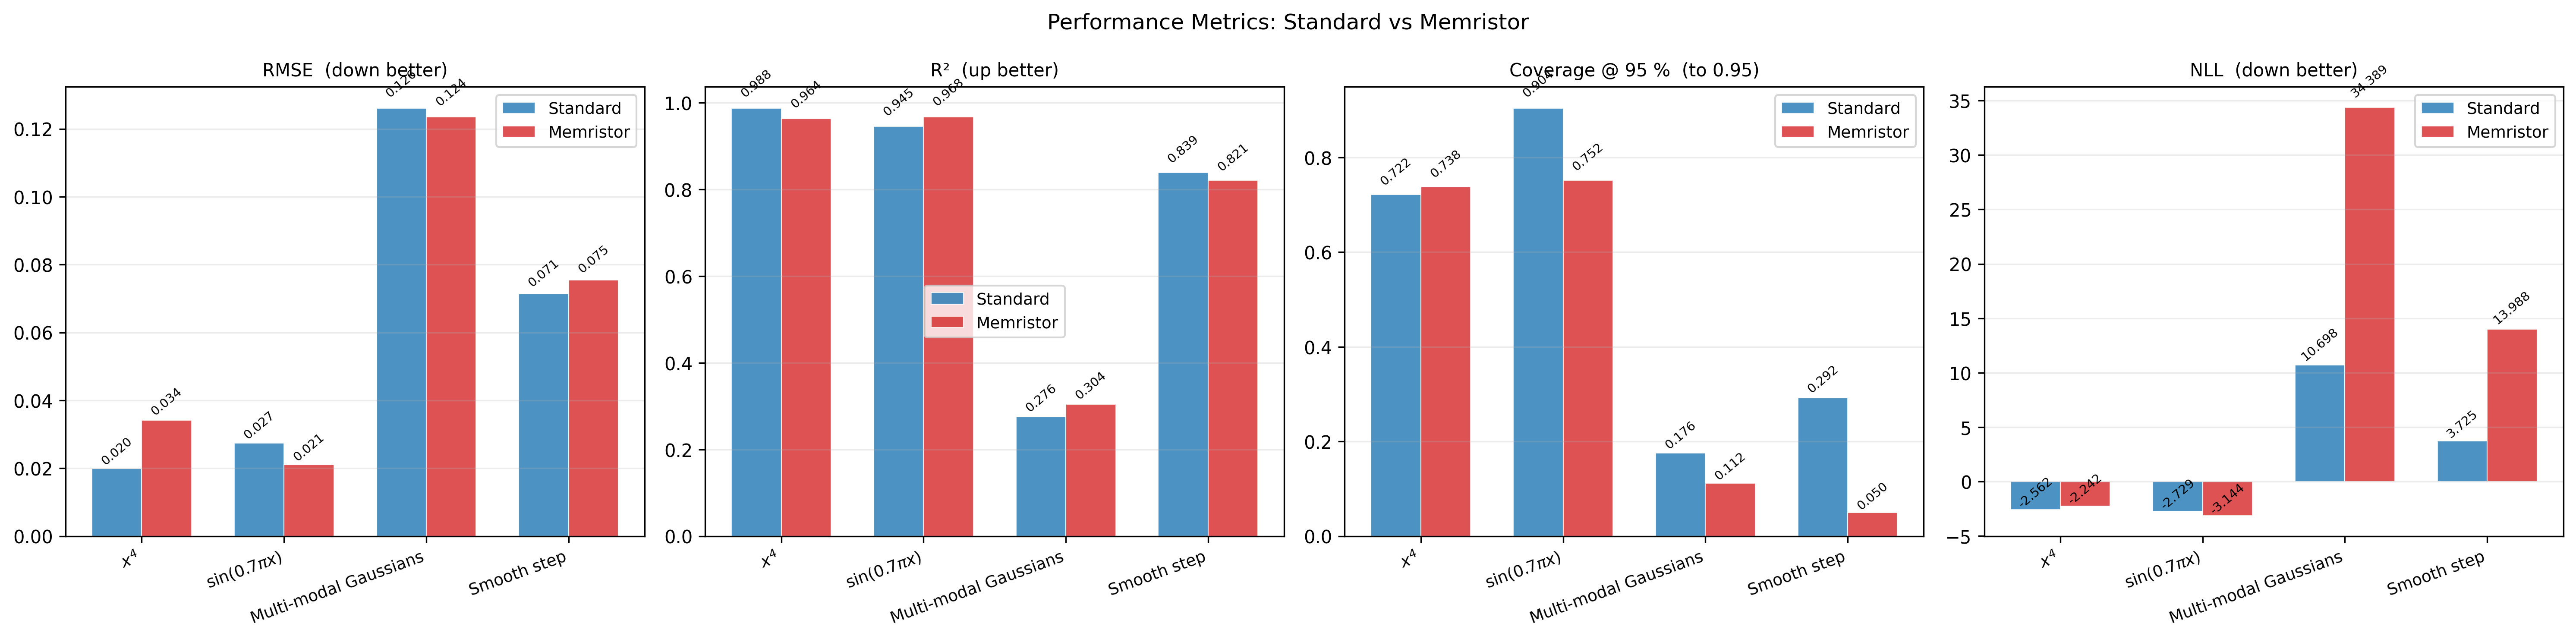
\includegraphics[width=0.95\textwidth]{../reports/function_and_memristor_comparison/2026-04-01_212859/metrics_comparison.png}
\end{frame}

\begin{frame}{Smooth-Step Placement Sweep}
\begin{table}
\centering
\begin{tabular}{lrrr}
\toprule
Placement & RMSE & $R^2$ & Coverage \\
\midrule
Standard & 0.0718 & 0.8377 & 0.368 \\
Phase 0 & 0.4038 & -4.1344 & 0.002 \\
Phase 2 & 0.0712 & 0.8403 & 0.278 \\
Phase 4 & 0.0712 & 0.8403 & 0.278 \\
Phase 6 & 0.0757 & 0.8193 & 0.048 \\
Phase 8 & 0.0712 & 0.8403 & 0.278 \\
\bottomrule
\end{tabular}
\end{table}

\begin{itemize}
    \item Placement matters a lot.
    \item Phase 0 is catastrophic.
    \item Phases 2/4/8 are close to baseline.
    \item Phase 6 is consistently harmful on smooth step.
\end{itemize}
\end{frame}

\begin{frame}{Smooth-Step Placement Fits}
    \centering
    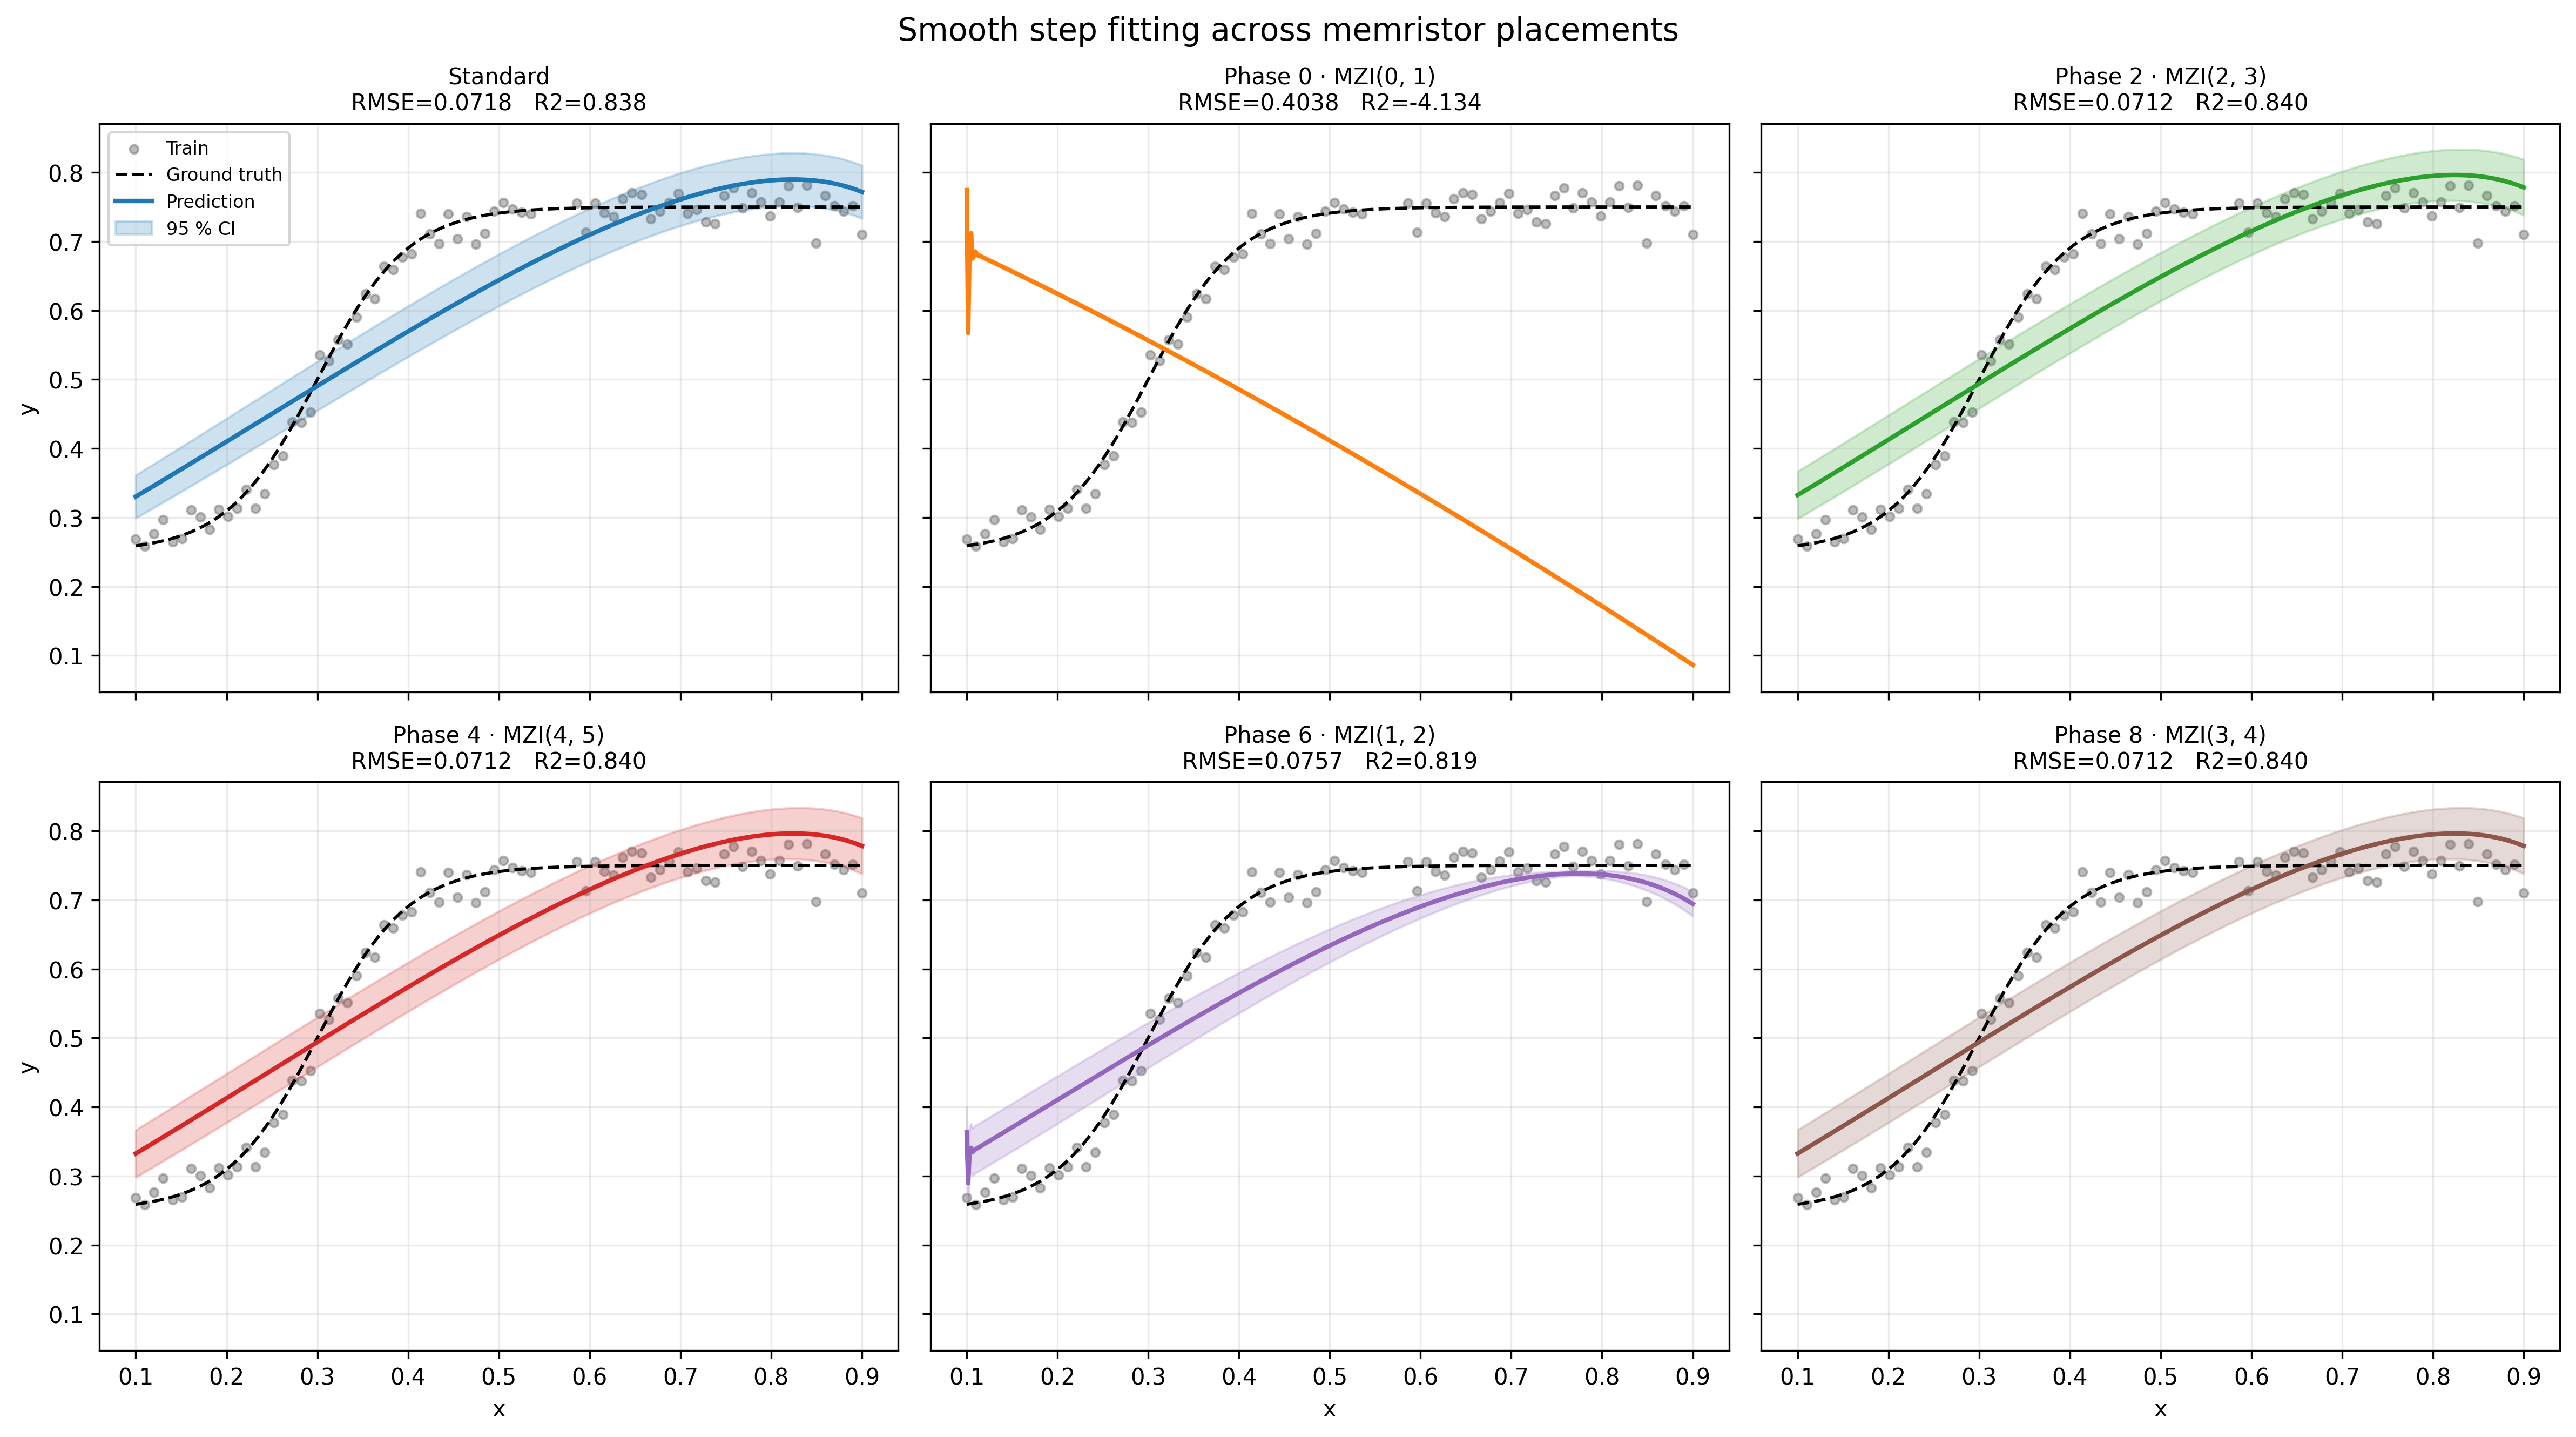
\includegraphics[width=0.95\textwidth]{../reports/smooth_step_memristor_placement_comparison/2026-04-01_223609/predictions_grid.png}
\end{frame}

\begin{frame}{One vs Two Memristors}
\begin{table}
\centering
\begin{tabular}{lrrrr}
\toprule
Config & RMSE & $R^2$ & Coverage & NLL \\
\midrule
Standard & 0.0718 & 0.8377 & 0.368 & 3.790 \\
Single 6 & 0.0757 & 0.8193 & 0.048 & 14.559 \\
Single 8 & 0.0712 & 0.8403 & 0.278 & 3.766 \\
Double 6+8 & 0.0764 & 0.8164 & 0.052 & 12.595 \\
\bottomrule
\end{tabular}
\end{table}

\begin{itemize}
    \item Adding a second memristor at phase 6 does not help.
    \item The best smooth-step result remains standard or single phase 8.
    \item ``More memristors'' is not the same as ``better fit.'' 
\end{itemize}
\end{frame}

\begin{frame}{Multiple-Memristor Comparison}
    \centering
    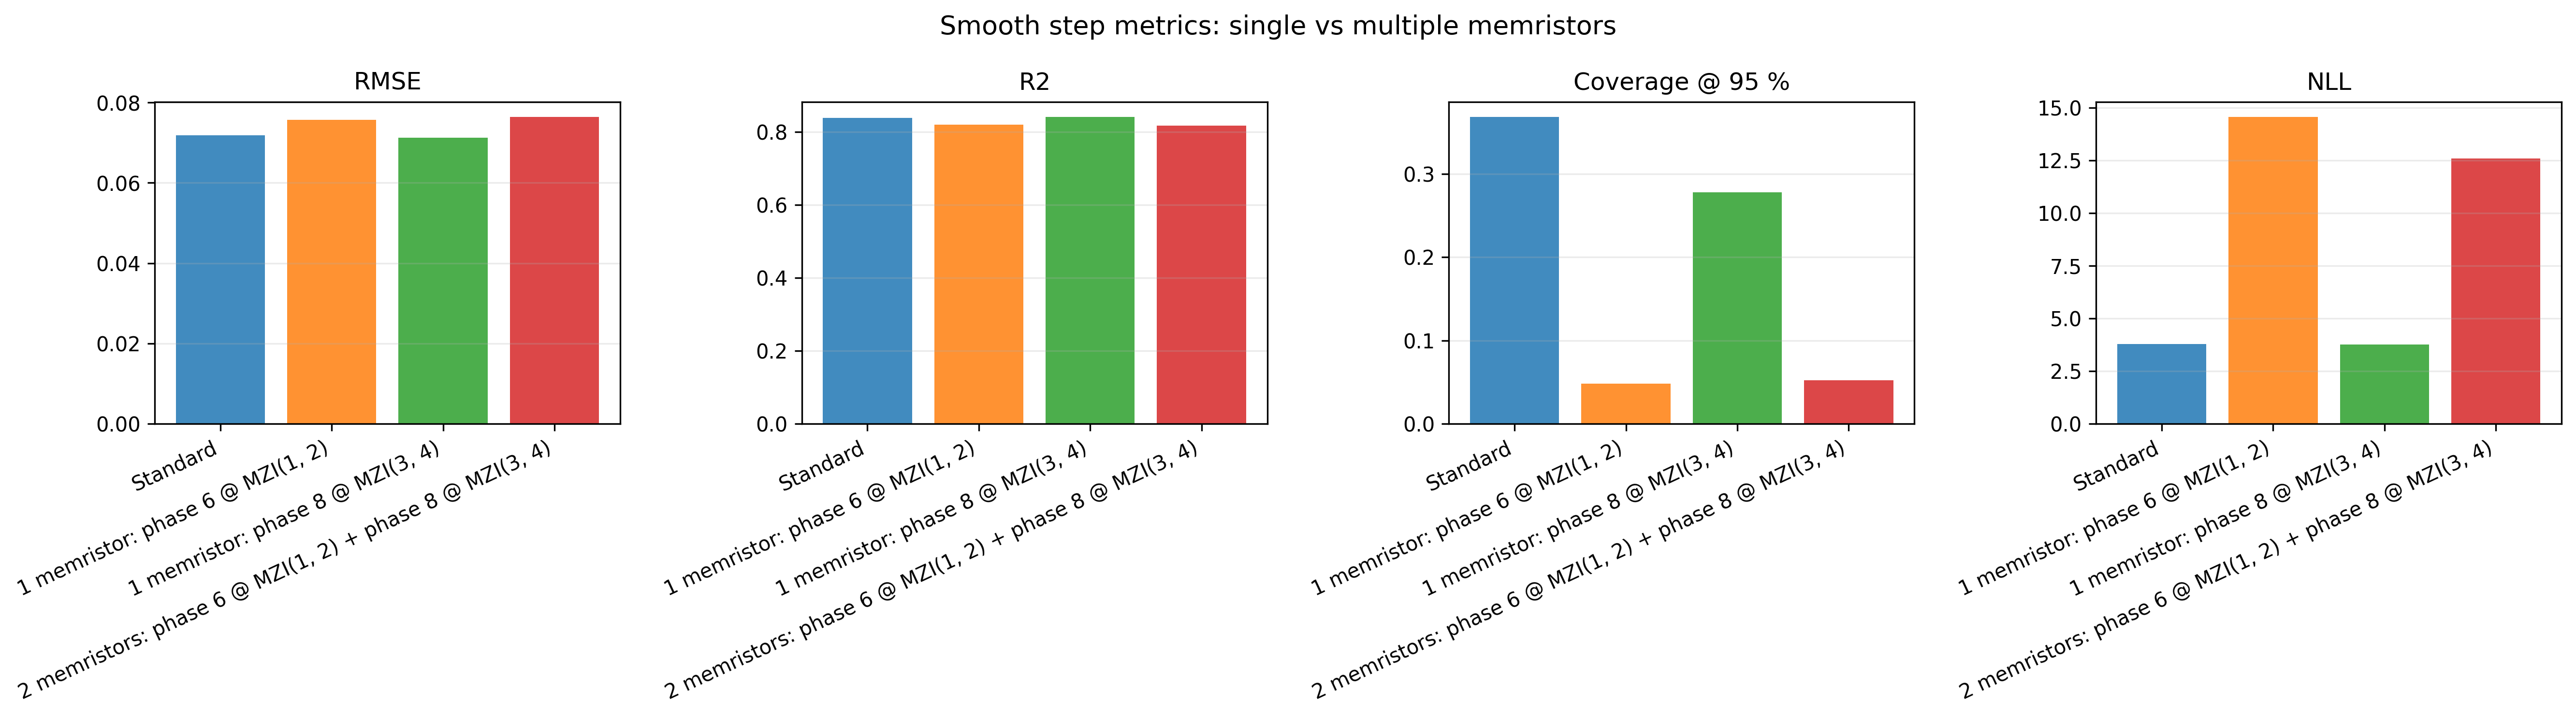
\includegraphics[width=0.95\textwidth]{../reports/smooth_step_multi_memristor_comparison/2026-04-01_230245/metrics_comparison.png}
\end{frame}

\begin{frame}{Backend Benchmark}
\begin{table}
\centering
\begin{tabular}{lrrr}
\toprule
Case & Fast [ms] & Legacy [ms] & Speedup \\
\midrule
Discrete & 5.562 & 22.994 & 4.13x \\
Swipe & 23.315 & 109.183 & 4.68x \\
Swipe inline & 22.744 & 100.722 & 4.43x \\
\bottomrule
\end{tabular}
\end{table}

\begin{itemize}
    \item The new memristive NumPy backend is about 4x--5x faster.
    \item The speedup is large enough to make rerun studies practical.
    \item Numerical parity with the old path was preserved by tests.
\end{itemize}
\end{frame}

\begin{frame}{Benchmark Plot}
    \centering
    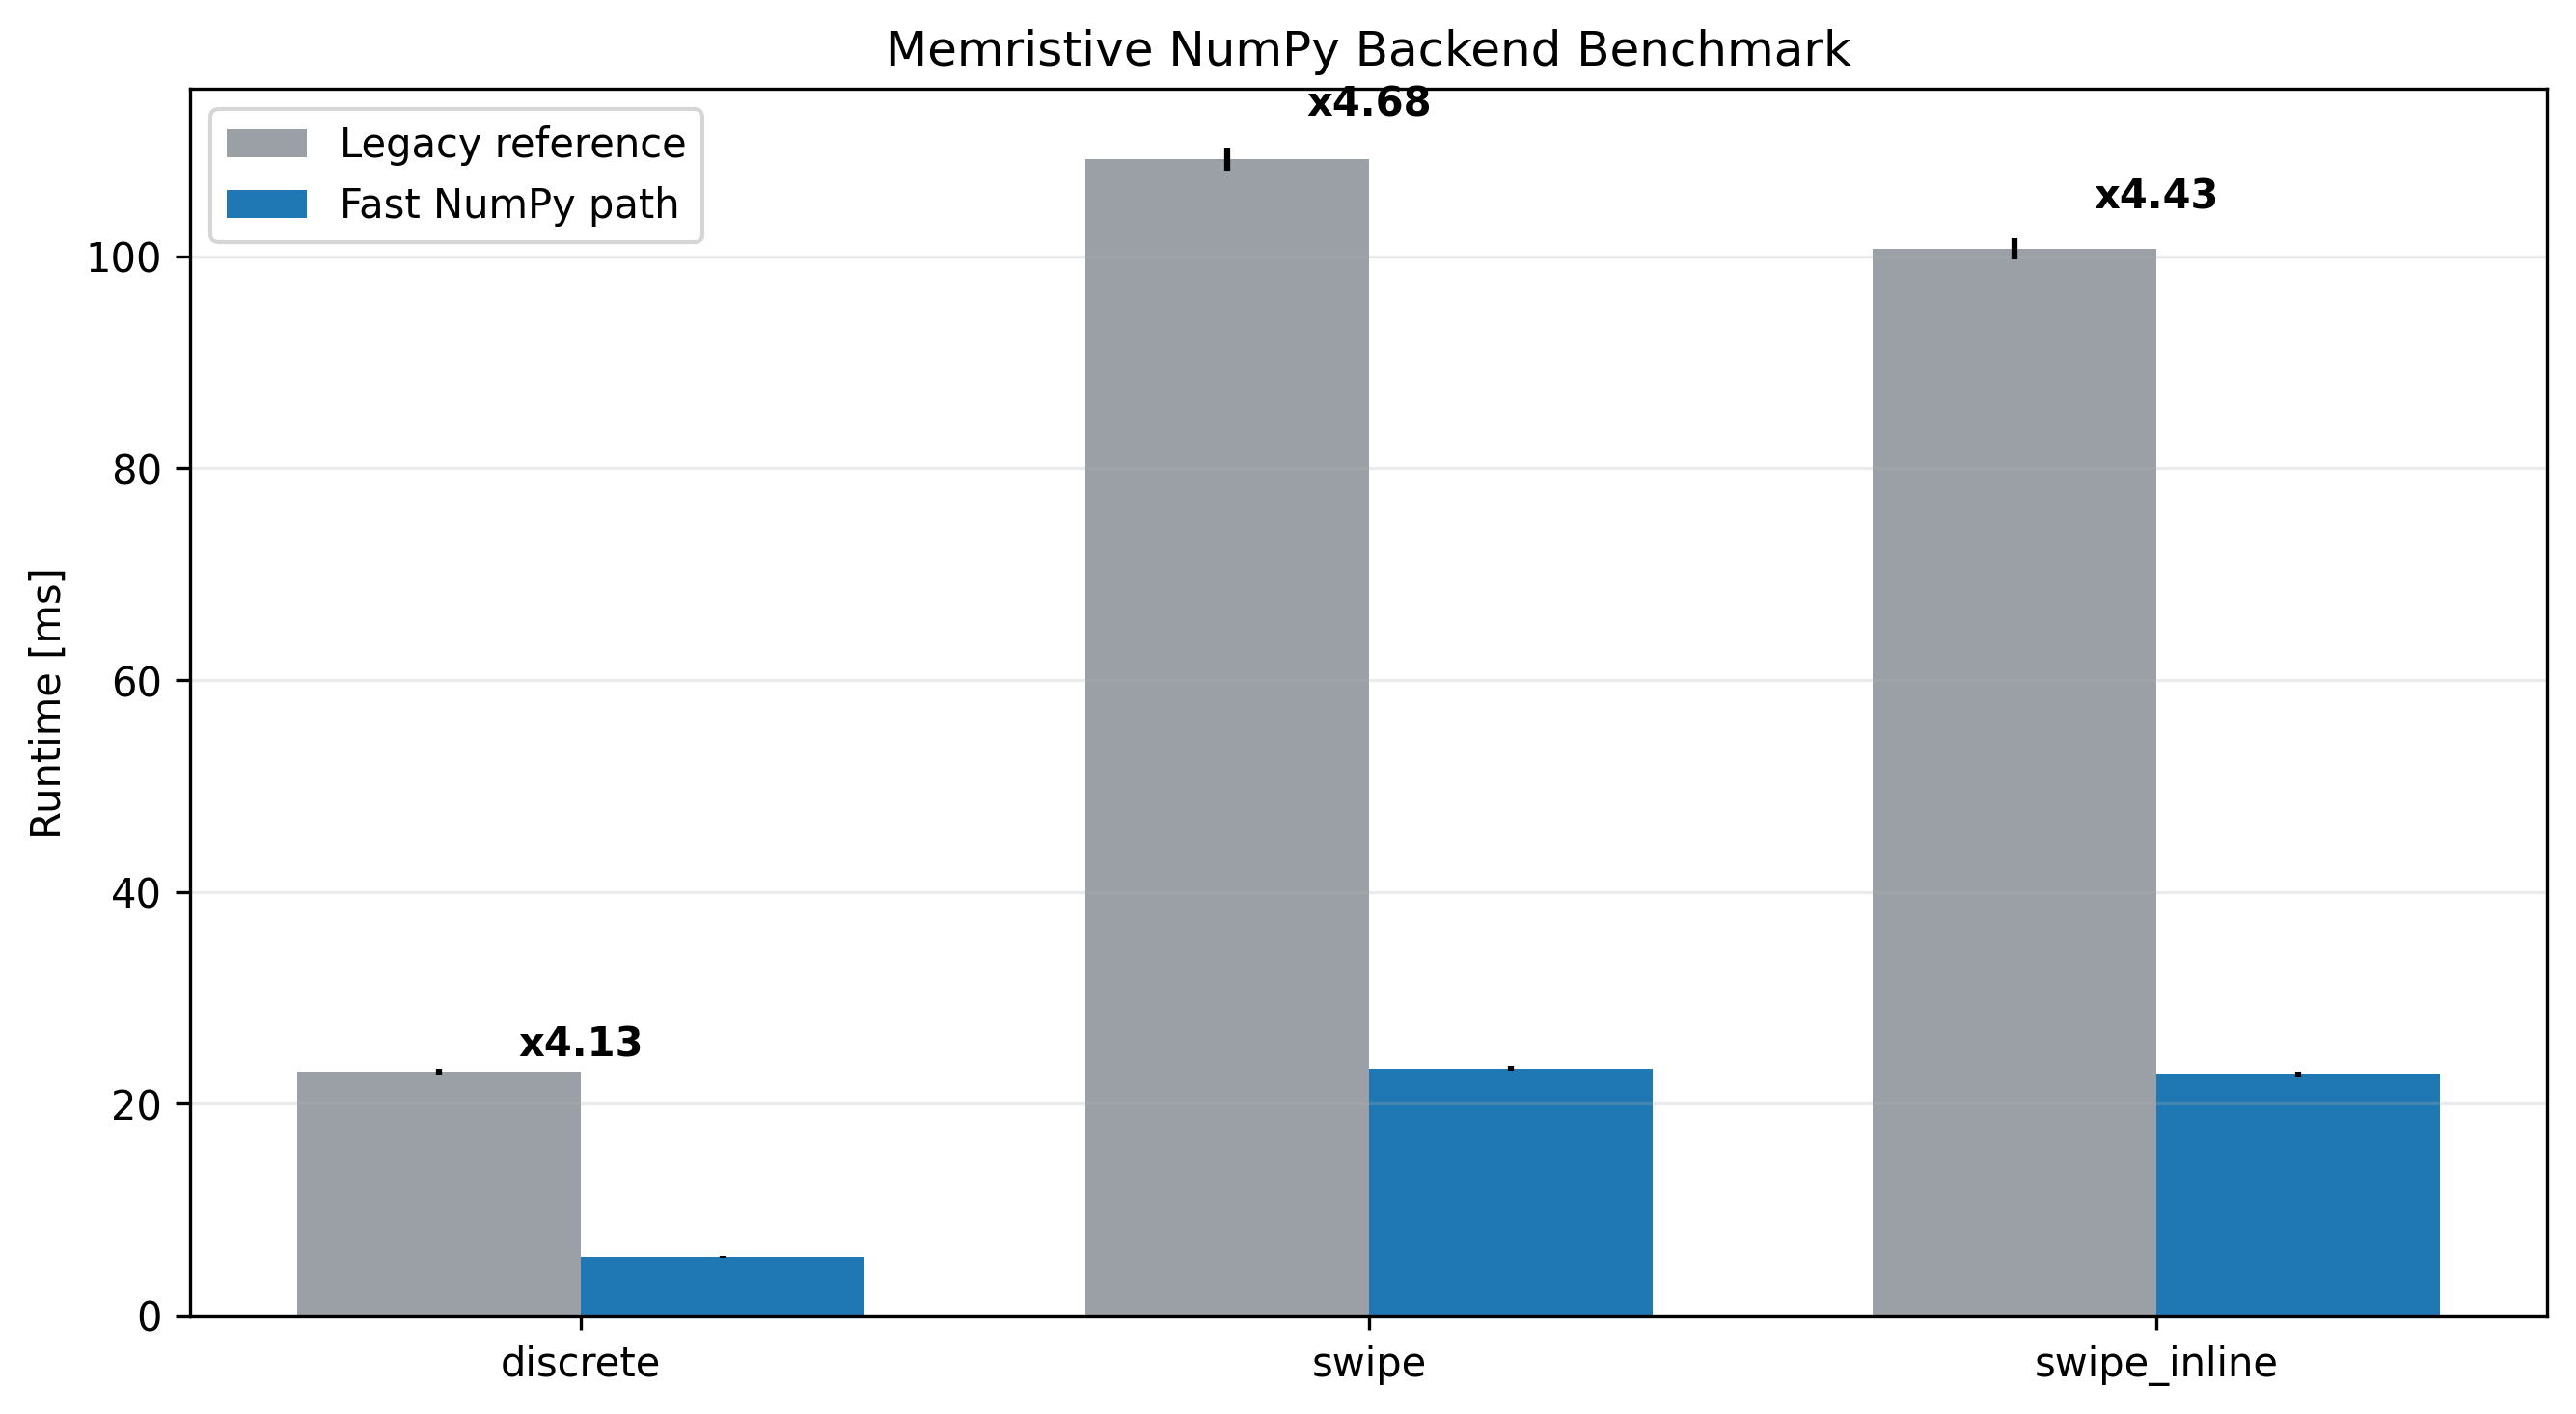
\includegraphics[width=0.82\textwidth]{../reports/memristive_backend_benchmark/2026-04-01_215523/memristive_backend_benchmark.png}
\end{frame}

\begin{frame}{Final Assessment}
\begin{block}{Engineering result}
The repository is now more reproducible, more modular, and significantly faster for memristive singles reruns.
\end{block}

\begin{block}{Scientific result}
Memristive feedback is task- and placement-dependent. It can help some targets, but on smooth-step fitting the tested placements and the tested two-memristor pair did not outperform the standard baseline in a robust way.
\end{block}

\begin{block}{Next step}
Search better multi-memristor pairs, vary memory depth, and test harder functions where temporal-style feedback may be more useful.
\end{block}
\end{frame}

\end{document}
